\documentclass[aps,prl,twocolumn,nofootinbib]{revtex4-1}
\usepackage{graphics,color,graphicx,amsmath}
\usepackage{xr,natbib}
\bibliographystyle{vancouver}
\usepackage{amsbsy}

\newcommand{\norm}[1]{\left\Vert#1\right\Vert}
\newcommand{\abs}[1]{\left\vert#1\right\vert}
\newcommand{\set}[1]{\left\{#1\right\}}
\newcommand{\Real}{\mathbb R}
\newcommand{\eps}{\varepsilon}
\newcommand{\To}{\longrightarrow}
\newcommand{\BX}{\mathbf{B}(X)}
\bibliographystyle{unsrt}
\graphicspath{{images}}

\begin{document}

% COMMANDS -------------------------------------------------------
\newcommand{\mr}[1]{\mathrm{#1}}
\newcommand{\mb}[1]{\mathbf{#1}}
\newcommand{\br}[1]{\left<#1\right>}
\newcommand{\bl}[1]{\left|#1\right|}
\newcommand{\mc}[1]{\mathcal{#1}}
\newcommand{\tb}[1]{\textcolor{blue}{#1}}
\newcommand{\tr}[1]{\textcolor{red}{#1}}
\newcommand{\tg}[1]{\textcolor{green}{#1}}
\newcommand{\si}[0]{\sigma_{\rm i}}
\newcommand{\sj}[0]{\sigma_{\rm j}}
\newcommand{\bs}[1]{\boldsymbol{#1}}
\newcommand{\rs}[0]{{\rm s}}
\newcommand{\rk}[0]{{\rm k}}

\title{CONvenient Interface to Inverse Ising (CONIII): A Python package for solving maximum entropy models}
\author{$^1$Edward D Lee, $^2$Bryan C Daniels}
\affiliation{$^1$Department of Physics, 132A Clark Hall, Cornell University, Ithaca NY 14850, $^2$ASU--SFI Center for Biosocial Complex Systems, Arizona State University, Tempe, AZ 85287}

\begin{abstract}
CONIII is an open-source Python project providing a simple interface to solving maximum entropy models, with a focus on the Ising model. We describe the maximum entropy problem and give an overview of the algorithms that are implemented as part of CONIII (\url{https://github.com/bcdaniels/coniii}) including a regularized mean field method, Monte Carlo histogram, pseudolikelihood, and minimum probability flow. We briefly explain how one should approach and validate maxent models from the perspective of model selection. Our goal is to make a variety of maximum entropy techniques accessible to those unfamiliar with the techniques and accelerate workflow for users.
%We then show examples of models that have been solved on various data sets using CONIII.
\end{abstract}

\maketitle

\section{Introduction}
Many biological and social systems are characterized by collective behavior: the correlated pattern of neuron firing \cite{Schneidman:2006he}, protein diversity in the immune system \cite{XXX}, conflict participation in monkeys \cite{XXX}, flocking in birds \cite{Bialek:2012cs}, statistics of letters in words \cite{XXX}, or consensus voting in the US Supreme Court \cite{Lee:2015ev}. Statistical physics is a natural approach to probing such systems precisely because they are collective \cite{Castellano:2009ce}.
Recently, the development of numerical, analytic, and computational tools have made it feasible in these large collective systems to solve for the statistical model that reproduces system behavior, corresponding to solving an ``inverse problem''.
This approach contrasts with the typical problem in statistical physics where one postulates the microscopic model (the Hamiltonian) and works out the physical behavior of the system. In the \textit{inverse} problem, we  find the parameters that correspond to observed behavior of a known system. In many cases, this is a very difficult problem to solve and does not have an analytical solution, and we must rely on analytic approximation and numerical techniques to estimate the parameters.

The Ising model has been of particular interest because of its simplicity and generality. A variety of algorithms have been proposed to solve the inverse Ising problem, but different approaches are disparately available on separate code bases in different coding languages, which makes comparison difficult and pedagogy more complicated.
CONIII (Convenient Interface to Inverse Ising) is a Python project intended to provide a centralized resource for the inverse Ising problem and provide a base for the addition of more maximum entropy problems in the future. With CONIII, it is possible to solve the inverse Ising problem with a variety of algorithms in just a few lines of code.
%The modular structure of CONIII was inspired by the machine learning package scikit-learn, where each algorithm is implemented in a class.
%There are a variety of techniques for approaching the inverse problem|often in context of a particular model|but they are often presented as different approaches without clear relations to one another. Instead of focusing on the details of each technique separately, we relate these techniques to one another and point out when one would fail or be difficult to apply.

%We hope to provide a (soft) introduction to the analytic, numerical, and computational techniques used to solve these problems to make them accessible to students especially at the graduate level in physics and beyond (and even advanced undergraduates). With the goal of furthering general understanding, we aim not to be rigorous but to be accurate and comprehensible, pointing to the relevant literature whenever possible. Although we strive to be as clear and explicit as possible across this guide, a good background in mathematics or physics will be extremely helpful. In some places, we have left out steps in the derivations, and we encourage the reader to work out the missing steps.

\section{What is maximum entropy?}
Shannon introduced the concept of information entropy in his seminal paper about communication over a noisy channel \cite{Shannon:1948wk}. Information entropy is the unique measure of uncertainty that follows from insisting on some elementary principles of consistency. According to Shannon, the entropy over the probability distribution $p(s)$ of possible discrete configurations $s$ of a system is\footnote{Technically speaking, this is the ``information entropy''.}
\begin{align}
	S[p] &= -\sum_{{\rm s}\in \mathcal{S}} p({\rm s}) \log p({\rm s}).
\end{align}
These configurations could be on-off patterns of firing in neurons, the arrangement of 4 letters in a word, or the orientation of spins in a material.

When there is no structure in the distribution, meaning that the probability is uniform ($p(s) = p(s')$ for all $s$ and $s'$), entropy is at a maximum. In the context of communication theory as Shannon first discussed, this means that there is no structure to exploit to make a prediction about the next part of an incoming message; thus, maximum entropy means that each new part of the message is maximally ``surprising.'' At the other extreme, when the message consists of the same bit over and over again, we can always guess at the following part of the message and the signal has zero entropy. In the context of modeling, we use entropy not to refer to the difficulty of the message, but to our state of knowledge about it. Entropy precisely measures our uncertainty about which configuration $s$ we will see next.

Maximum entropy, or maxent, is the formal framework for building models that are consistent with statistics from the data but otherwise as structureless as possible \cite{Bretthorst:2003ua,Jaynes:1957fy}.
This is a constrained maximization problem. From the data set, we compute some useful feature $f_{\rm k}(\rm s)$ over all the observations in the data set ${\rm s}\in\mathcal{D}$. In a stochastic setting, this value will not always be the same, so we compute the average of the feature,
\begin{align}
	\br{f_k}_{\rm data} &= \frac{1}{R}\sum_{s\in \mathcal{D}} f_k({\rm s})
\end{align}
According to the model in which each observation s occurs with some probability $p(\rm s)$, the same average is calculated over all possible states
\begin{align}
	\br{f_{\rm k}} &= \sum_{\rm s\in\mathcal{S}} p(\rs)f_{\rm k}(\rs)
\end{align}

We assert that the model should fit the $K$ features while maximizing entropy. The standard procedure is to solve this by the method of Langrangian multipliers. We construct the Langrangian functional $\mathcal{L}$ by introducing the multipliers $\lambda_{\rm k}$.
\begin{align}
	\mathcal{L}[p] &= -\sum_{\rm s} p(\rs)\log p(\rs) - \sum_k^K \lambda_k \left(\br{f_{\rm k}}-\br{f_{\rm k}}_{\rm data}\right)\label{eq:Lagrang}
\end{align}


%In the notation of statistical physics, the Langrangian is the Helmholtz free energy describing the competition between entropy and the structure described in the Hamiltonian $E$ in equilibrium (See Appendix) \footnote{If we fix the average energy of the system, we get the microcanonical ensemble (See Appendix). which is equivalent to the axiom that all microstates have equal probability (that is the maxent distribution).}.
%\begin{align}
%	F &= S - \br{E}\\
%	E &= -\sum_{\rm k}^K\lambda_{\rm k}f_{\rm k}(s)
%\end{align}
%This formulation makes clear the fundamental connection that statistical mechanics is an inference procedure using the maximum entropy principle \cite{Jaynes:1957fy}.

Then, we solve for the fixed point by taking the derivative with respect to $\lambda_{\rm k}$.
The resulting model is a Boltzmann distribution over states:
\begin{align}
    \label{eq:energy}
	p_{\rm ME}(s) &= \left.e^{-E(s)}\right/Z,\\
\intertext{with relative negative log-likelihood (also known as the energy or Hamiltonian)}
E(s) &= -\sum_{\rm k}^K\lambda_{\rm k}f_{\rm k}(s),
\intertext{and normalization factor (also known as the partition function)}
	Z &= \sum_{\rm s} e^{-E(s)}.
\end{align}
Readers familiar with statistical physics will recognize this as a derivation of the microcanonical ensemble, demonstrating that statistical mechanics can be viewed as an inference procedure using the maximum entropy principle \cite{Jaynes:1957fy}.

Finding the parameters $\lambda_k$ that match the constraints $\br{f_k}_{\rm data}$ is equivalent to minimizing the Kullback-Leibler divergence between the model and the data \cite{Cover:2006tl}
\begin{align}
	D_{KL}(p_{\rm data}||p_{\rm ME}) &= \sum_s p_{\rm data} \log\left(\frac{p_{\rm data}(s)}{p_{\rm ME}(s)}\right);\\
	\frac{\partial D_{KL}}{\partial \lambda_k} &= \sum_s p_{\rm data}(s) \frac{\partial (-E(s)-\log Z)}{\partial \lambda_k} = 0 \nonumber \\
	\implies  \br{f_k}_{\rm data} &= \br{f_k}_{\rm ME}\label{eq:fk-fk}.
\end{align}
[Of course, we also have to show that the problem is convex.] In other words, the parameters of the maximum entropy model are the ones that minimize the information theoretic ``distance'' to the distribution of the data. Note that these parameters are given by the data: once the constraints have been chosen, there is a single maximum entropy solution, with no free parameters.

\subsection{Ising model}
The Ising model is a statistical physics model of magnetism \cite{Ising:1924vf}. It consists of a set of spins $\sigma_{\rm i}$ with 2 possible orientations (up and down), each coupled to an external magnetic field $h_{\rm i}$ and coupled to each other with couplings $J_{\rm ij}$. The strength of the magnetic field determines the tendency of each of the spins to orient in a particular direction and the couplings $J_{\rm ij}$ determine whether the spins tend to point together ($J_{\rm ij}>0$) or against each other ($J_{\rm ij}<0$). Typically, neighbors are defined as spins that interact with one another given by some underlying network structure: Figure \ref{gr:ising} shows a fully-connected example.

\begin{figure}[tbp]\centering
	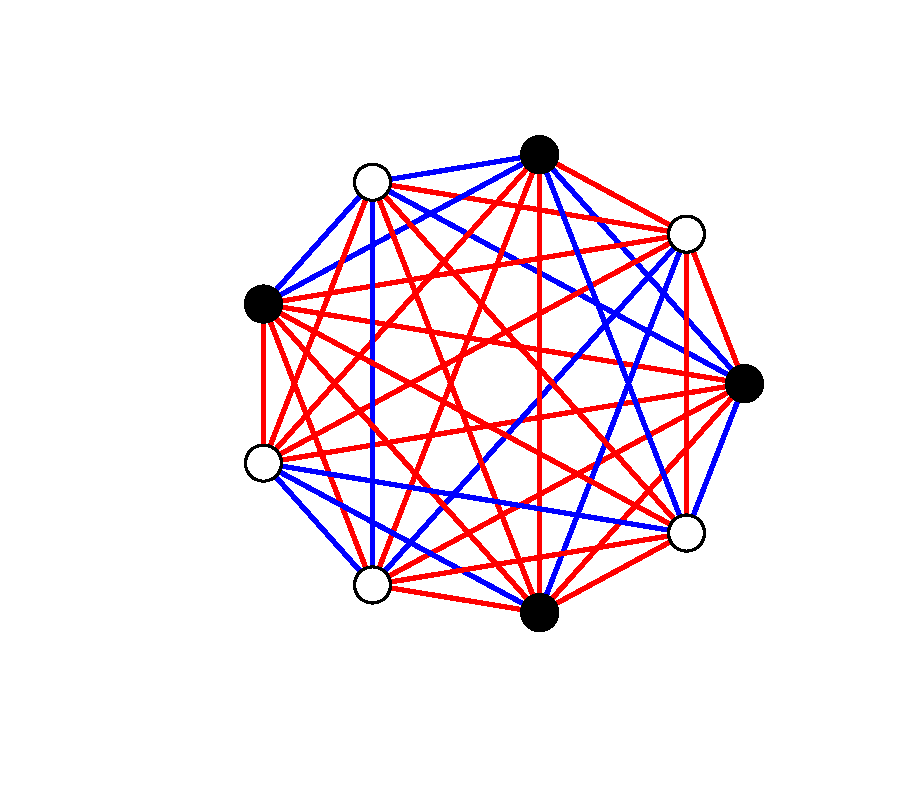
\includegraphics[width=.85\linewidth,clip,trim={100 70 70 60}]{../images/ising_example}
\caption{Example of a fully connected Ising model with random couplings. Each spin $\si$ (circle) can take one of two states (black or white, corresponding to $-1$ and $+1$) and is connected to every other spin in the system with a positive or negative coupling.  This schematic represents one possible state of the spins.  The inverse Ising problem starts with statistics about the states observed in the system and infers the coupling strengths $J_{ij}$ and individual biases $h_i$ that produce such statistics. }
\label{gr:ising}
\end{figure}

The energy of each configuration determines its probability via \eqref{eq:energy}:
\begin{align}
	E &= -\sum_{\rm \br{ij}} J_{\rm ij}\si\sj -\sum_{\rm i=1}^Nh_{\rm i}\si.
\end{align}
%States with lower energy are more likely so spin tend to orient along the direction of the local field $h_{\rm i}^{\rm local} = \sum_{\rm j}J_{\rm ij}\sj +h_{\rm i}$. 

We can derive the Ising model from the perspective of maximum entropy. Fixing the the means and pairwise correlations to those observed in the data
\begin{align}
	\br{\si} &= \br{\si}_{\rm data} \\
	\br{\si\sj} &= \br{\si\sj}_{\rm data}
\end{align}
we go through the procedure of constructing the Langrangian from Eq~\ref{eq:Lagrang}
\begin{align}
	\mathcal{L}[p] &= -\sum_s p(s)\log p(s) +\sum_{\rm \br{ij}} J_{\rm ij}\br{\si\sj} +\sum_{\rm i=1}^Nh_{\rm i}\br{\si}\\
	\frac{\partial\mathcal{L}[p]}{\partial p(s)} &= -\log p(s)-1 +\sum_{\rm \br{ij}} J_{\rm ij}\si\sj +\sum_{\rm i=1}^Nh_{\rm i}\si\\
	\log p(s) &= -1 +\sum_{\rm \br{ij}} J_{\rm ij}\si\sj +\sum_{\rm i=1}^Nh_{\rm i}\si\\
	p(s) &= \left.e^{-E(s)}\right/Z\\
\intertext{where to enforce normalization of the probability distribution $\sum_s p(s) = 1$,}
	Z &= \sum_s e^{-E(s)}.
\end{align}
Thus, the resulting model is exactly the Ising model mentioned earlier.

Despite the simplicity of the Ising model, the structure imposed by the discrete nature of the spins means that finding the parameters is challenging analytically and computationally. In the last few years, numerous techniques have been suggested for solving the inverse Ising problem exactly or approximately \cite{Nguyen:2017ww}. We have implemented some of them in CONIII and designed a package structure to make it easily extensible to include more methods.  Here, we briefly describe the algorithms that are part of the first official version of the package. The goal is to give the user a sense (or reminder) of how they work without getting bogged down in heavy detail. For more detail, we suggest perusing the papers referenced in each section or the review \cite{Nguyen:2017ww}. For a complete beginner, it may be useful to first get familiar with a slower introduction like in the Appendix of Ref \cite{Lee:2015ev}, Ref \cite{Bialek:2012ueb}, or Ref \cite{Bretthorst:2003ua}.

%Imagine that you have a system with $n$ components that have been sampled many times. To be more specific, we'll take $n=9$ voters on the US Supreme Court that either vote with in the majority, the winning coalition, or in the minority. [More generally, we could think some like gene expression levels in a cell a coarse-grained representation where relatively high or low expression can be represented by a binary variable. Of course, we don't have to restrict ourselves to binary variables \cite{Lezon:2006ws}.]
%The primary difficulty for solving probabilistic models is calculating the normalization because of the size of the state space. Most of the methods below involve avoiding that problem in the first place (Monte Carlo sampling, MCH) or approximations to drastically reduce the state space (pseudolikelihood, adaptive cluster expansion).


\section{Enumeration}
The na\"{i}ve approach that only works for small systems is to write out the equations from Eq~\ref{eq:fk-fk} and solve them numerically. After writing out all $K$ equations,
\begin{align}
	\br{f_{\rm k}}_{\rm data} &= \br{f_{\rm k}}\\
	\br{f_{\rm k}}_{\rm data} &= -\frac{\partial \ln Z}{\partial \lambda_{\rm k}},
\end{align}
we can use any standard optimization algorithm to find the parameters $\lambda_{\rm k}$. 
This approach, however, involves enumerating all terms in the partition function $Z$ whose number grows exponentially with system size. 
%[Simple example with logical gates?]

For the Ising model, the first step in the algorithm for writing down the equations is $\mathcal{O}(K^2 2^{N})$ where $K$ is the number of constraints and $N$ the number of spins. In the second step, each evaluation of the objective in the minimization algorithm will be of the same order. For relatively small systems $n\leq15$, however, this approach is feasible on a typical desktop computer and is a good way to test the results of a more complicated algorithm.

This approach is part of the {\tt Exact} class that contains code for writing Eqs~\ref{eq:fk-fk} into a file and solving them with the {\tt scipy.optimize} library.


\section{Monte Carlo method}
Perhaps the most straightforward and most expensive computational approach is to use Monte Carlo Markov Chain (MCMC) sampling to approximate the distribution and adjust the parameters appropriately after each step. The parameters are adjusted using a learning rule, and both sampling and learning are repeated til the stopping criterion is met.
%The magic behind MCMC approaches is that only relative probabilities of states need to be known to return a sample of the distribution. Thus, we do not need to calculate the partition function, but can instead compute the difference in energy between two states. 
This can be combined with a variety of approximate gradient descent methods to reduce the number of sampling steps. The particular technique implemented in CONIII is the Monte Carlo Histogram (MCH) method \cite{Broderick:2007wq}.

Since the sampling step is expensive, the idea behind MCH is to reuse a sample for more than one gradient descent step because we can predict how the distribution will change if we modify the parameters slightly \cite{Broderick:2007wq}. Given that we have a sample with probability distribution $p(\rs)$ generated with parameters $\lambda_{\rm k}$, we would like to estimate the new distribution $p'(\rs)$ from adjusting our parameters $\lambda_{\rm k}' = \lambda_{\rm k}+\Delta\lambda_{\rm k}$. We can leverage our current sample to make this extrapolation.
\begin{align}
	p' &= \frac{p'}{p}p\\
	p'(\rs)	&= \frac{Z}{Z'}e^{\sum_\rk \Delta\lambda_k f_\rk(\rs)} p(\rs)\\
\intertext{To estimate the average,}
	\sum_s p'(\rs) f_{\rm k}(\rs) &= \frac{Z}{Z'} \sum_s p(\rs) e^{\sum_{\rm k} \Delta\lambda_{\rm k} f_{\rm k}(\rs)} f_{\rm k}(\rs)\\
\intertext{To be explicit about the fact that we only have a sampled approximation to $p$, we replace $p$ with the data distribution.}
	\br{f_{\rm k}}' &= \frac{Z}{Z'} \br{e^{\sum_{\rm k} \Delta\lambda_{\rm k} f_{\rm k}(\rs)} f_{\rm k}(\rs)}_{\rm sample}
\end{align}
Likewise, the ratio of the partition function can be estimated
\begin{align}
	\frac{Z}{Z'} \approx 1\left/\br{e^{\sum_{\rm k} \Delta\lambda_{\rm k} f_{\rm k}(\rs)}}_{\rm sample}\right.
\end{align}

At each step, we update the Lagrangian multipliers $\{\lambda_\rk\}$ while being careful to stay within the bounds of a reasonable extrapolation. One suggestion is to update the parameters with some inertia
\begin{align}
	\Delta\lambda_\rk(t+1) &= \Delta \lambda_\rk(t) + \epsilon \Delta\lambda_\rk(t-1)\label{eq:mch learn1}\\
	\Delta \lambda_\rk(t) &= \eta\left(\br{f_\rk}'-\br{f_\rk}\right)\label{eq:mch learn2}
\end{align}
This has the correct fixed points.
%Another heuristic is to begin with a small sample size and increase the size of the sample set as we refine our estimates of the parameters.

In practice, MCH can be difficult to tune properly and one must check in on the progress of the algorithm often. One issue is choosing how to set the learning rule parameters $\eta$ and $\epsilon$. One suggestion for $\eta$ is to shrink it as the inverse of the number of iterations \cite{Tkacik:2006vq}. Another issue is that parameters cannot be changed by too much when using the MCH approximation step or the extrapolation to $\lambda_{\rm k}'$ will be inaccurate and the algorithm will fail to converge. In CONIII, this can be controlled by setting a bound on the maximum possible change in each parameter  $\Delta\lambda_{\rm max}$ and restricting the norm of the vector of change in parameters $\sum_k \sqrt{\Delta\lambda_{\rm k}^2}$. Another issue is setting the parameters of the MCMC sampling routine. Both the burn time (the number of iterations before starting to sample) and sampling iterations (number of iterations between samples) must be large enough that we are sampling from the equilibrium distribution.  Typically, these are found by looking at the decorrelation time in the energy or correlations as a function of MCMC iterations made. The parameter may need to be updated during the course of MCH because the sampling parameters may need to change with the estimated parameters of the model. For some regime of parameter space, samples are correlated over long times and alternative sampling methods like Wolff or Swendsen-Wang should be used.
We do not discuss these sampling details here, but see Ref \cite{MacKay:2005wc,Newman:1999wu} for examples.

The main computation cost for MCH is the sampling step. The runtime is proportional to the number of samples $n_{\rm sample}$, number of MCMC iterations $n_{MC}$, the number of constraints $K$:
$\mathcal{O}(n_{\rm MC} n_{\rm sample} K)$, whereas the MCH estimate is relatively quick $\mathcal{O}(n_{\rm sample}n_{\rm MCH}K)$ because the number of MCH approximation steps is much smaller than the number of MCMC sampling iterations $n_{\rm MCH}<<n_{\rm MC}$. 
%What is the runtime for the learning rules Eqs \ref{eq:mch learn1} and \ref{eq:mch learn2}?
For the Ising model, $K\sim N^2$, the system size squared.

MCH is implemented in the {\tt MCH} class.

\section{Pseudolikelihood}
The pseudolikelihood approach is an analytic approximation to the likelihood that drastically reduces the computational complexity of the problem and is exact in the thermodynamic limit \cite{Aurell:2012hi}. We maximize the conditional probability of each spin $s_{\rm i}$ given the rest of the system
\begin{align}
	p\left(s_{\rm i}|{\bf s}_{\backslash \rm i}\right) &= \left( 1+e^{-2s_{\rm i} \left(h_{\rm i}+\sum_{j\neq i}J_{\rm ij}s_{\rm j}\right)} \right)^{-1}
\end{align}
Taking the logarithm and summing over all spins, we define the approximate likelihood to be summed over all data points indexed by $r$.
\begin{align}
	f(h_{\rm i},\bs{J}_{\rm i}) &= \sum_{\rm r=1}^R \ln p\left(\left.s_{\rm i}^{(r)}\right|\bs{s}_{\backslash\rm i}^{(r)}\right)
\end{align}
In the limit where the ensemble is well sampled, the average over the data can be replaced by an average over the ensemble
\begin{align}
	f(h_{\rm i},\bs{J}_{\rm i}) &= \sum_{\bs{s}} \ln p\left(\left.s_{\rm i}^{(r)}\right|\bs{s}_{\backslash\rm i}^{(r)}\right)p(\bs{s};h,J)\\
\intertext{At maximum likelihood,}
	\frac{\partial f}{\partial J_{\rm ij}} &= \sum_{\bs{s}} \ln p\left(\left.s_{\rm i}^{(r)}\right|\bs{s}_{\backslash\rm i}^{(r)}\right)p(\bs{s};h,J)=0
\end{align}

Pseudolikelihood is extremely fast. Each iteration only is $O(RN^2)$ and often surprisingly accurate.

We have implemented pseudolikelihood for the Ising model in {\tt Pseudo}.

\section{Minimum Probability Flow}
Minimum probability flow involves analytically approximating how the probability distribution \textit{changes} as we modify the \textit{configurations} \cite{Sohl-Dickstein:2009tt,SohlDickstein:2011im}. In the methods so far mentioned, the approach has been to maximize the objective (the likelihood function) by immediately taking the derivative with respect to the parameters. With MPF, we first posit a set of dynamics that will lead the data distribution to equilibrate to that of the model. When these distributions are equivalent, then there is no ``probability flow'' between them. This technique is closely related to score matching where instead we have a continuous state space and can directly take the derivative with respect to the states without specifying dynamics \cite{Hyvarinen:2007ed}.

As before, we start with minimizing the Kullback-Leibler divergence, but instead of taking the derivative with respect to the parameters, we first ask how the probability flows between the model and the states in the data $\mathcal{D}$ if the dynamics are run for an infinitesimal amount of time $\epsilon$, the idea being that the relative difference between the probability distributions are minimized with optimal parameters.
\begin{align}
	\partial_t D_{KL}(p^{(0)}||p^{(t)}\left(\{\lambda_k\}\right)) &= \sum_{\rm s \not\in \mathcal{D}} \dot{p}_{\rm s}(\lambda_k)\\
	K(\{\lambda_{\rm k}\}) &= \sum_{\rm s \not\in \mathcal{D}} \dot{p}_{\rm s}(\lambda_k)
\end{align}

Monte Carlo dynamics (satisfying ergodicity and detailed balance) would lead to equilibration of the two distributions. A simple transition matrix suggested in Ref \cite{SohlDickstein:2011im} is
\begin{align}
	\dot{p}_{\rm s} &= \sum_{s'\neq s} \Gamma_{\rm ss'} p_{\rm s'} -\sum_{\rm s'\neq s} \Gamma_{\rm s's} p_{\rm s}\\
	\Gamma_{\rm ss'} &= g_{\rm ss'}\exp\left[ \frac{1}{2}\left( E_{\rm s'}-E_{\rm s} \right) \right]
\end{align}
with transition probabilities $\Gamma_{\rm ss'}$ from state ${\rm s'}$ to state s. The connectivity matrix $g_{\rm ss'}$ specifies whether there is edge between states s and ${\rm s'}$ such that probability can flow between them. By choosing a sparse $g_{\rm ss'}$ while not breaking ergodicity, we drastically reduce the computational cost of calculating the objective function.

Finally, we must find the minimum of the objective function
\begin{align}
	K(\{\lambda_{\rm k}\}) &= \sum_{\rm s \not\in \mathcal{D}} \dot{p}_{\rm s}(\lambda_k)
\end{align}

%MPF satisfies a number of useful properties:

At each step of the algorithm for the Ising model, the runtime is $O(RN^2)$.

MPF is implemented in the {\tt MPF} class.

\section{Mean-field method}
One attractively simple and efficient version of the regularized approach starts
with mean-field theory.  In the inverse Ising problem, mean-field theory is equivalent
to treating each binary individual as instead having a continuously varying state
(corresponding to its mean value).  The inverse problem then turns into simply inverting
the correlation matrix $C$ \cite{CocMon12}:
\begin{equation}
\label{meanFieldSolution}
J^{\mathrm{mean-field}}_{\rm ij} =
    - \frac{ (C^{-1})_{\rm ij} }{ \sqrt{p_{\rm i}(1-p_{\rm i})p_{\rm j}(1-p_{\rm j})} },
\end{equation}
where
\begin{equation}
C_{\rm ij} = \frac{ p_{\rm ij} - p_{\rm i} p_{\rm j} }{ \sqrt{p_{\rm i}(1-p_{\rm i})p_{\rm j}(1-p_{\rm j})} },
\end{equation}
and where $p_{\rm i}$ corresponds to the frequency of individual i being
in the active ($+1$) state and $p_{\rm ij}$ is the frequency of the pair
i and j being simultanously in the active state.

A simple regularization scheme in this case is to discourage large values in the interaction
matrix $J$.  This corresponds to putting more weight on solutions that are closer to
the case with no interactions (independent individuals).  A particularly convenient form
adds the following term, quadratic in $J$, to the negative log-likelihood:
\begin{equation}
\gamma \sum_{\rm i} \sum_{\rm j > i} J_{\rm ij}^2 p_{\rm i} (1-p_{\rm i}) p_{\rm j} (1-p_{\rm j}).
\end{equation}
In this case, the regularized version of the mean-field solution in \eqref{meanFieldSolution}
can be solved analytically, with the slowest computational step coming from the inversion
of the correlation matrix.  For details, see Refs.~\cite{Daniels:1cq,BarCoc13}.

The idea is then to vary the regularization strength $\gamma$ to move between the
non-interacting case ($\gamma \rightarrow \infty$) and the naively calculated
mean-field solution \eqref{meanFieldSolution} ($\gamma \rightarrow 0$).
While there is no guarantee that varying this one parameter will produce solutions that are
good enough to ``fit within error bars,'' this approach has been successful in at least
one case of fitting social interactions \cite{Daniels:1cq}.

This is implemented in {\tt RegularizedMeanField}.



\section{Cluster expansions}

Adaptive cluster expansion \cite{Monasson:2011fo,CocMon12,BarCoc13}
iteratively calculates terms in the
cluster expansion of the entropy $S$:
\begin{equation}
S = \sum_\Gamma \Delta S_\Gamma,
\end{equation}
where the sum is over clusters $\Gamma$ and in the exact case
includes all $2^N - 1$ possible nonempty subsets of individuals in the system.\footnote{In the simplest version of the expansion,
one expands around $S=0$.  In some cases it can be more advantageous to write the
expansion around $S-S_0$, where $S_0$ is a reference entropy corresponding to
an easily calculated case such as
the independent individual solution or one of the mean-field solutions
described in the previous section \cite{BarCoc13}.}
The inverse Ising problem is solved independently
on each of the clusters, which can be done exactly when the
clusters are small.  These results are used to construct a full
interaction matrix $J$.
The expansion starts with small clusters and expands to use larger
clusters, neglecting any clusters whose
contribution $\Delta S_\Gamma$ to the entropy falls below a threshold.
To find the best solution that does not overfit,
the threshold is initially set at a large value and then lowered,
gradually including more clusters in the expansion, until samples from
the resulting $J$ fit the desired statistics of the data sufficiently well.

In CONIII, the selective cluster expansion method is implemented in the {\tt ClusterExpansion} class.

%\section{Bethe/Kikuchi free energy/cavity methods}
%Another approach involves a cluster-expansion of the free energy, also known as the cavity method. This has not yet been implemented in CONIII.
%The cavity method involves use of the marginalized distribution.

%\section{Incomplete data}

\section{Samplers}
In CONIII, we have implemented two versions of the Metropolis algorithm. One is specific to the Ising model {\tt MCIsing} and the other {\tt MC} can sample a system as long as the function for calculating the energy is supplied by the user.

In some parameter regimes, where spins are tightly correlated, the Metropolis algorithm is very inefficient. Cluster sampling like Wolff or Swendsen-Wang are much more efficient.

%\section{Algorithm for solving}
%We suggest solving the inverse problem using a fast technique. 

\section{Model fitting}
A fundamental problem in model inference is that uncertainty coming
from the finiteness of data translates into uncertainties in parameters.
In the exposition of the maxent formulation derived from Eq~\ref{eq:Lagrang}, there is no fitting of the model parameters because they are given by the data once the constraints are specified. In reality, constraints are typically estimated from a finite sample, and they are noisy.
The straightforward answer to this problem is to take more data---in a pairwise
maximum entropy problem, we might insist that we have enough samples to well-constrain
the correlation between every pair of individuals.  But it is not always possible
to take enough data.  For instance, in a social system in which we are trying to
measure stable social structure that lasts on the order of months, there are only
a finite number of social interactions that occur over those months, which may
not be enough to tightly constrain parameters. When we fit to the exactly measured constraints, we run the danger of overfitting and poor generalization in the limit of small data.

When we find the parameters that minimize the Kullback-Leilber divergence between the model and the data distributions, we are maximizing the likelihood of the data. 
Around the peak in likelihood, sample size fluctuations will determine some curvature of the likelihood curve around the maximum.
This uncertainty is reflected in the sample size fluctuations we can easily calculate from the data. Assuming that the data is independently and identically distributed, the errors are given by the standard error of the mean of a binomial distribution \mbox{$p_{\rm ij...k} = p(s_{\rm i}=s_{\rm j}=...=s_{\rm k}=1)$} with $K$ data points.
\begin{align}
	\delta_{\rm ij...k} &= \sqrt{(1-p_{\rm ij...k})p_{\rm ij...k}/K}
\end{align}
In other words, we are not obliged to keep pushing the parameters to get closer to the data once we have gotten close enough, where close enough is given by the noise the data distribution.\footnote{This is like early stopping \cite{}.}

An alternative approach is to regularize the problem like with the regularized mean field or cluster expansion algorithms. Here, we restrict the search space in some principled way so that more complicated
solutions are disallowed.  We then check that the regularized solutions fit the
data within expected statistical fluctuations.  If not, a more lax regularization
can be used to allow more complicated solutions that are able to fit the
remaining signal in the data. 
In the Bayesian formulation, this approach is equivalent to including a prior distribution over the parameters
\begin{align}
	\log p({\rm model}|{\rm data}) &\propto \log p({\rm data}|{\rm model}) + \log p({\rm model})\label{eq:prior}
\end{align}

\section{Model Validation}
Besides just fitting the model while accounting for the noisiness of the data, how do we know if we need a more complicated model? To answer this question, we need a way of quantifying the tradeoff between the complexity and fit of the model. 

When we search for the peak in the posterior probability of the data, we must account for the balance between a good description of the data with the cost of describing the model. This tradeoff manifests as the competition between the likelihood and prior on the model's parameters in the Bayesian formulation of the problem in Eq~\ref{eq:prior}. Roughly speaking, we can imagine that specifying the $L$ parameters is localizing a region in a high-dimensional space where each dimension shrinks with the number of data points $K$ as $\sim K^{-1/2}$. The volume of the ``ball'' grows like $K^{-L/2}$, so that the information cost goes like $-\frac{L}{2}\log(K)$ \cite{Lee:2015ev}. This is the picture formalized by quantities like the Akaike information criterion (AIC) or the Bayesian information criterion (BIC) \cite{Anonymous:mVL3xTtr}.

Although likelihood tells us how well the models are doing relative to one another, it does not tell us in detail how the model is fitting the data.
Basic checks would be to compare against any other correlations in the data.
% In Figure~??, we show an example of a pairwise maxent model tested against higher order correlations. 
Since these are quantities averaged over the joint probability distribution of many spins, a stricter check would be to compare the entire probability distribution of the pairwise maxent model with that of the data \cite{Lee:2015ev}, but this is only feasible when the data set is reasonably large. 
A more specific test would be against features that are relevant to the question at hand. For conflict in monkeys, a coarse-grained feature is the distribution of conflict sizes which seems to have a characteristically long tail, and that is checked specifically \cite{Daniels:1cq}. 

A summary of how well the model captures the distribution across the entire probability distribution is the multi-information. If we take a maxent model and add further constraints, the models can be ordered in terms of entropy $S_{\rm 1}>S_{2}>...S_{\rm m}>...>S_{\rm data}$, where the minimum entropy the most constrained model could have is equal to the data. To measure how much correlation in the data our model has captured, we can calculate the multi-information $I_{\rm m} = S_{\rm 1}-S_{\rm m}$, the amount of correlation captured by the model relative to the independent model. The fraction of multi-information captured is $F=I_{\rm m}/I_{\rm data}$. This is a measure of how much of the correlation in the data is captured by the model.\footnote{See Refs \cite{Bialek:2012ueb} and \cite{Lee:2015ev} for details and further references on how to estimate information quantities.}

Choosing which constraints to impose is an important question. Typically, the approach is to constrain the lowest order interactions that are sufficient to produce collective behavior. The intuition from physics is from the observation that many physical systems are extremely well (if not exactly) described by pairwise interactions.\footnote{In statistical physics, highly correlated behavior across space and time can emerge from pairwise interactions and renormalization group flow ensures they are the only relevant parameters in the thermodynamic limit \cite{}.} In fact, just the observation that we can model a system well with only pairwise interactions may be surprising \cite{Ranganathan:2007wz}. From the model fitting perspective, however, we might choose to constrain other parts of the probability distribution. In Ref \cite{Ganmor:2011ct}, they explore choosing correlations to constrain depending on whether or not they are signicantly large. In Ref \cite{Nemenman:2016kl}, they discuss how a pairwise model becomes an increasingly effective description of a system with higher order interactions as the system gets larger.



\section{Conclusion}
Science is a process of model selection. In the ideal picture, we start with the simplest models and the fewest constraints possible, and then we increase the complexity of the model til it is sufficiently so to make good predictions. In principle, we could add as many contraints as would allow us to fit the data well, but the idea is that complex models are not only ``expensive'' but they do not generalize well.
Maxent is a principled framework for this picture of model building. The number of parameters and the order of the constraints we impose can be adjusted to test our hypotheses about what matters for the system.
In this sense, the maxent approach is a useful ``model'' framework for thinking about statistical inference problems far beyond statistical physics. We build an open-source Python package that we hope will be accessible and useful for those unfamiliar with maxent approaches to experiment and perhaps apply this technique to their questions.


%\section{The microcanonical ensemble and maximum entropy}
%The conventional textbook in statistical mechanics first introduces the concept of entropy as a way of counting the phase volume available to the system at a given energy
%\begin{align}
%	S(E) &= k_B \log\Omega(E)
%\end{align}
%where $k_B$ is Boltzmann's constant and $\Omega$ the number of states between $E$ and $E+\delta E$. Temperature is defined as
%\begin{align}
%	\frac{1}{T} &= \frac{\partial S}{\partial E}
%\end{align}
%
% begins with the concept of a small system coupled to a heat bath. In this limit, we can linearly expand thermodynamic quantities about the energy of the bath $E_{\rm bath} = E-E_s$
%\begin{align}
%	S_{\rm bath}(E-E_s) &\approx S_{\rm bath}(E) -E_s\left.\frac{\partial S}{\partial E_s}\right|_{E-E_s}\\
%		&= S_{\rm bath}(E) -\frac{E_s}{T}\\
%	e^{S_{\rm bath}(E-E_s)/k_B} &= e^{S_{\rm bath}(E)/k_B} e^{-E_s/k_BT}
%\intertext{Since the entropy is proportional to the density of states at a particular energy $E_s$, Eq ?? corresponds to}
%	p(E_s) &= e^{-E_s/k_BT}/Z
%\end{align}
%With partition function $Z$. In other words, the Gibbs measure takes exponential form. Eq ?? can be rewritten in terms of free energy
%\begin{align}
%	\log p(E_s) &= -E_s/k_BT -\log(Z)
%\intertext{Averaging both sides over all energy configurations and rearranging}
%	-k_B T\log Z &= \sum_s p(E_s) E_s +k_BT\sum_s p(E_s)\log p(E_s)
%\intertext{Remembering the fundamental postulate of statistical mechanics that all states are equally likely}
%	-k_BT\log Z &= \br{E_s} - TS\\
%	F &= \br{E_s} -TS
%\end{align}
%This equation tells us how the Helmholtz free energy is related to the internal energy and the entropy of the system.
%
%When we say that free energy is minimized for a system with Hamiltonian $E_s$ at equilibrium, we are equivalently saying that entropy is maximized. Entropy maximization is the crux of statistical physics models.

\bibliography{refs}

\end{document}  
